The magnetic field $\boldsymbol{B_p}$ of a mobile device without iron effects can be described with roll $\phi$, pitch $\theta$ and $\psi$ as the equation:
\begin{equation} \label{eq:magnField}
  \boldsymbol{B_p} = 
  \boldsymbol{R_x}(\phi)\boldsymbol{R_y}(\theta)\boldsymbol{R_z}(\psi)\boldsymbol{B_r} = 
  \boldsymbol{R_x}(\phi)\boldsymbol{R_y}(\theta)\boldsymbol{R_z}(\psi)B\begin{pmatrix}cos(\delta) \\ 0  \\ sin(\delta)\end{pmatrix}
\end{equation}
with the rotations where $ \boldsymbol{R_x}(\phi)$,$\boldsymbol{R_y}(\theta)$ and $\boldsymbol{R_z}(\psi)$ is the rotation matrices, $\boldsymbol{B_r}$ is the local geomagnetic field vector with magnitude $B$ and the magnetic tilt $\delta$. The hard iron offset can be described as the vector $\boldsymbol{V_{PCB}}$ which will according to ~\cite{sensor:magnIron} appear additive to the vector of the sensor $\boldsymbol{V_{Sensor}}$. This gives the equation:
\begin{equation}
\end{equation}
~\cite[]{sensor:magnIron}

  When looking at devices with similar or same hardware you can see differences in measurements, for example here are the accelerometer recordings from 5 iPhone 6 and 1 iPhone 5S:
\begin{figure}[H]
\centering
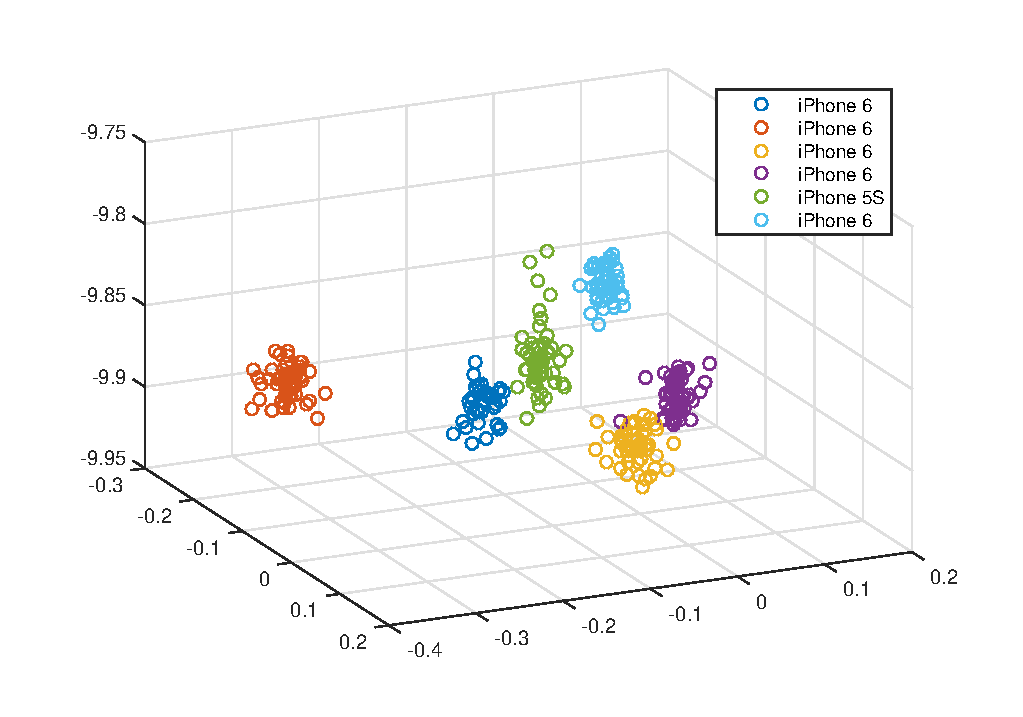
\includegraphics[scale=.6]{img/scatteriPhone}
\caption{Scatter graph on accelerometer recordings of 6 Apple devices}
\label{fig:digraph}
\end{figure}